\subsection{Angelo Parrinello}
Il mio compito all’interno del progetto è stato quello di modellare il \texttt{GameLoop}, le statistiche della partita ed infine mi sono occupato delle \texttt{Wave} (ondate di nemici) insieme a Penazzi. Inoltre, ho provveduto a sviluppare componenti di \texttt{Model} gestiti dal \texttt{GameLoop} quali \texttt{MetaData} e \texttt{GameData}, che si occupano rispettivamente della gestione di dati trasversali alla partita e di manipolare le entità in gioco. Infine, ho collaborato a stretto contatto con il team per implementare aspetti e funzionalità comuni di \texttt{Model}, \texttt{Controller} e \texttt{View}.

\subsubsection{GameLoop}
Il \texttt{GameLoop} è il componente che si occupa di aggiornare il \texttt{Model} e il successivo \textit{refresh} della \texttt{View}. Nel nostro contesto, il \texttt{GameLoop} si occupa anche di aggiornare il \texttt{Model} a seguito di una richiesta da parte dell'utente (es: piazzare una nuova torretta).\\
\\La funzione principale è quella di \textit{Update} del sistema. Tipicamente questo avviene attraverso un ciclo che richiama rispettivamente l'aggiornamento del \texttt{Model} e della \texttt{View}. Nel paradigma ad attori questo comportamento non è ammissibile in quanto si andrebbe a creare un \textit{handler bloccante}, bloccando il \textit{flusso interno} di controllo, facendo perdere reattività all'attore. L'attore emula questa comportamento utilizzando i \texttt{TimerScheduler} proprietari di \textit{Akka}: allo scadere di questo timer, l'attore invia un messaggio a sè stesso di tipo \texttt{UpdateLoop} ed infine ricrea il timer con un certo \textit{delay}. Il \texttt{GameLoop} alla ricezione della richiesta di aggiornamento, notifica gli attori del \texttt{Model} ed, in seguito alla risposta di quest'ultimi, aggiornerà la \texttt{View} con i dati rivisti. Di seguito viene schematizzato tale comportamento.

\begin{figure}[H]
    \centering
    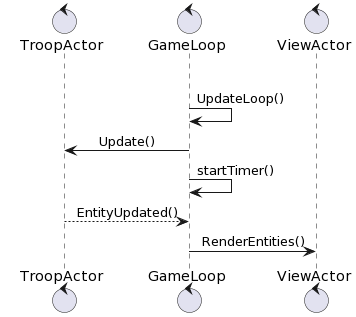
\includegraphics[width=0.61\linewidth]{images/game-update.png}
    \caption{Diagramma di sequenza della fase di Update del gioco.}
\end{figure}
Non entrerò nel dettaglio di altre sequenze di sistema che comprendono il \texttt{GameLoop} essendo abbastanza intuitive o che sono state implementata seguendo scelte già fatte (es: la fase di \textit{Update} delle risorse/soli del gioco che utilizza la stessa logica legata al \texttt{TimerScheduler}).\\

Il design del gioco assume che solo il \texttt{GameLoop} abbia coscienza dello stato intero del gioco, quindi esclusivamente lui conterrà tutte le informazioni ad esso associate. Una di queste è la \textit{sequenza} di entità, in un prefissato momento, nel gioco e la corrispondente parte reattiva. Durante lo sviluppo mi son reso conto che utilizzare delle semplici sequenze di \textit{tuple} non era l'ideale. Il codice risultante presentava diversi difetti quali \textit{ripetitività} e \textit{opacità}. Dopo aver vagliato diverse ipotesi, ho creato una \textbf{case class} che racchiudesse le informazioni relative al \texttt{Model} di un'entità e il riferimento al suo attore (chiamata \texttt{GameEntity} e \textbf{generica} in un sottotipo di \texttt{Entity}). In seguito, decisi di sfruttare il pattern funzionale \textbf{Pimp-my-library} convertendo le \texttt{Seq} in \texttt{GameSeq} (sequenze di \texttt{GameEntity}) con una \textbf{given conversion}.

\begin{lstlisting}[language=Scala, label=code:gamedata, caption=Parte del GameSeq.]
    given Conversion[Seq[GameEntity[Entity]], GameSeq] = 
        GameSeqImpl(_)

    /** Defines a [[GameSeq]] ... */
    trait GameSeq:
      /** Creates a [[Seq]] ... */
      def of[E <: Entity : GameSelectorBuilder]: Seq[GameEntity[E]] 
      = seq.collect(summon[GameSelectorBuilder[E]].by)

      /** Deletes a [[GameEntity]] ... */
      @targetName("delete")
      def :-(ref: ActorRef[ModelMessage]): Seq[GameEntity[Entity]] 
      = seq filter (_.ref != ref)
\end{lstlisting}

Questa scelta mi ha poi portato a creare un mini-\textbf{DSL} per creare in maniera elegante e funzionale sequenze di \texttt{GameEntity} definendo solo il tipo. L'idea di base dietro l'implementazione era avere \textbf{strategy} che definisse come una sequenza di \texttt{GameEntity} dovesse venire filtrata in base ad un tipo definito in input. Questo concetto, largamente sfruttato nella programmazione ad oggetti, vede un'analogia funzionale e idiomatica nei \textbf{contex-bounds}. Il metodo \texttt{of}, partendo dalla sequenza iniziale e sfruttando le \textbf{given instances}, genera così una nuova sequenza con solo gli elementi del tipo prestabilito.

\begin{lstlisting}[language=Scala, label=code:gameselector, caption= Creazione di una sequenza di gioco di soli tipi Troop.]
def of[E <: Entity : GameSelectorBuilder]: Seq[GameEntity[E]] =
    seq.collect(summon[GameSelectorBuilder[E]].by) 
    .
    .
 /** Contains some ways of creating [[GameSeq]]. */
  object GameSelector:
    /** Filters the [[GameEntity]] whose type is [[E]].
     *
     * @tparam E the type to filter.
     */
    trait GameSelectorBuilder[E <: Entity]:
      def by: PartialFunction[GameEntity[Entity], GameEntity[E]]

    given GameSelectorBuilder[Troop] with
      override def by: PartialFunction[GameEntity[Entity],               GameEntity[Troop]] = {
            case e if e.entity.isInstanceOf[Troop] => 
                GameEntity(e.ref, e.entity.asInstanceOf[Troop])
            }
\end{lstlisting}




Infine, il mio lavoro sul \texttt{GameLoop} mi ha portato ad introdurre il concetto di \textit{Collision}, di \textit{MetaData} e ad un utility object con funzionalità cardine per il controller di gioco. Nel caso delle collisioni, è stato interessante escogitare un metodo per rendere queste le più astratte possibili. In fase di modellazione mi è tornato utile il concetto delle \textbf{abstract types}. Infatti, in un primo momento sapevo che le collisioni sarebbero avvenuti tra due oggetti di tipo anche diverso, ma non erano stati definiti. Così facendo, le specifiche collisioni (al momento solo una) potranno essere definite più avanti nel tempo. Sempre rimanendo in tema collisioni, un altro punto importante è stato cercare una maniera \textit{idiomatica} e più \textit{funzionale} possibile per controllare in un'unico passaggio tutte le collisioni in un dato istante; \texttt{checkCollision} era stato implementato inizialmente con una serie di \textit{foreach}, \textit{map} e \textit{flatmap} ma, durante lo sviluppo, mi accorsi che così facendo il codice diveniva \textit{oscuro} ad un primo sgaurdo, più difficile da elaborare ed \textit{error-prone}. La scelta è quindi ricaduta sull'utilizzo di una \textbf{for-comprehension}, che aggiungendo lo \textit{zucchero sintattico} necessario, rendeva il tutto più chiaro e fluente.

\begin{lstlisting}[language=Scala, label=code:checkcollision, caption= Metodo che controlla e crea le collisioni.]
/** Detects [[Collision]] ... */
  def checkCollision(entities: Seq[GameEntity[Entity]]): 
    Seq[BulletTroopCollision] =
        for
            b <- entities.of[Bullet]
        yield
            BulletTroopCollision(b, for
                e <- entities.of[Troop]
                if b.entity isCollidingWith e.entity
            yield e)
\end{lstlisting}







\subsubsection{Statistiche}
Le \textit{Statistiche} sono quelle informazioni importanti per l'utente riguardo la partita appena svolta. Questi dati sono raccolti man mano che la partita avanza, tramite il \texttt{GameLoop}. In principio, sono stati definite quali statistiche andassero create. In generale, si è convenuto che le tre macro-tematiche dovessero essere: informazioni generali (es: numero di rounds) e informazioni su \texttt{Plant}/\texttt{Zombie} (es: numero di zombie uccisi). Quindi, ho ragionato su come il \texttt{GameLoop} dovesse manutenerle e in quali occasioni andassero aggiornate. Questo secondo step mi ha fatto capire che la struttura delle statistiche, così come quella dei \texttt{MetaData}, dovesse essere del tutto \textbf{immutabile}. Un uso sistematico di oggetti immutabili porta a codice più \textit{comprensibile} ed a facilitare la fase di \textit{debugging}. In fase implementativa, sono stati create tre \textit{Traits} ognuno con un compito specifico:
\begin{itemize}
    \item \texttt{GameStats}: definisce le informazioni di carattere generale sul gioco;
    \item \texttt{ZombieStatsOps}: definisce delle informazioni specifiche agli \texttt{Zombie};
    \item \texttt{PlantStatsOps}: definisce delle informazioni specifiche alle \texttt{Plant}.
\end{itemize}
Il concetto appena descritto era perfettamente adattabile al contesto dei \textbf{self-types} e \textbf{mixins}: concettualmente infatti è corretto che le informazioni relative agli \texttt{Zombie}/\texttt{Plant} venissero derivate solo utilizzando i dati generali. Inoltre, è possibile ottenere una sorta di ereditarietà (ma senza i problemi ad esso legati) e rappresentare questi concetti come \textit{decorazioni} componibili.

\begin{lstlisting}[language=Scala, label=code:statistics, caption=Statistiche relative agli Zombie.]
  /**
   * Defines which [[Zombie]]'s insights we want to gather from the game.
   */
  trait ZombieStatsOps:
    stats: GameStats =>
    /**
     *
     * @return the [[Zombie]]s killed.
     */
    def getZombies: Seq[Zombie] =
      stats.entities.foldLeft(List.empty)((acc, e) => e match {
        case zombie: Zombie => acc :+ zombie
        case _ => acc
      })
\end{lstlisting}



\subsubsection{Wave}
La parte che sono in procinto di spiegare, è stata modellata e sviluppata in modalità di \textbf{pair-programming} con il collega Penazzi Paolo. Per ragioni di impaginazione abbiamo deciso di inserirla sotto la mia sezione implementativa.\\

La \texttt{Wave} è una sequenza prestabilita di \textit{Zombie}. Le partite sono organizzate a \texttt{Wave}, che scandiscono il ciclo di vita del gioco. All'interno di una \texttt{Wave} possono essere presenti tutti i tipi di \texttt{Zombie} definiti nel gioco. I tipi e il numero degli \texttt{Zombie} che compongono la \texttt{Wave} determina la \textit{potenza} di quest'ultima. Con l'avanzare del gioco le \texttt{Wave} avranno una potenza sempre maggiore: comportamento incrementale tipico dei \textit{tower defense}. E' stato creato un oggetto \texttt{WaveGenerator} incaricato di generare le ondate di \texttt{Zombie}. Le ondate di \texttt{Zombie} possono essere generate in due modi:
\begin{itemize}
    \item Utilizzando \textbf{Scala}: in questa maniera si genera un'ondata di zombie composta solo da \texttt{BasicZombie}. L'ondata viene creata attraverso una funzione \textbf{tail recursive}.
    \begin{lstlisting}[language=Scala, label=code:tailrec-basiczombie, caption=Tail recursive Function per la creazione di Wave con Scala.]
  @tailrec
  private def createEnemyList(n: Int)(l: Seq[Zombie]): Seq[Zombie] =
    n match
      case 0 => l
      case _ => createEnemyList(n - 1)(l = l :+ BasicZombie())
\end{lstlisting}
    \item Utilizzando \textbf{Prolog}: in questa maniera si genera un'ondata di \texttt{Zombie} composta da qualsiasi tipo di nemico. Il processo sfrutta il \texttt{TuProlog Engine} per creare sequenze di tipi di \texttt{Zombie} casuali ma che rispecchino la potenza dell'ondata.
    \begin{lstlisting}[language=Prolog, label=code:prolog-theory, caption=Prolog Theory.]
% wave/2(+WavePower, -ListOfZombies)
% Returns a wave of zombies of the given power.
wave(0, []):- !.
wave(1, [1]):- !.
wave(2, [X|L]) :- random_zombie(2, X), M is 2 - X, wave(M, L), !.
wave(N, [X|L]) :- N > 2, random_zombie(3, X), M is N - X, wave(M, L).

% random_zombie/2(+MaxValue, -RandomNumber)
% Returns a RandomNumber between 1 and MaxValue.
% In this game each number is associated to a zombie.
random_zombie(Max, X) :- rand_int(Max, N), X is N + 1.
\end{lstlisting}
    Il predicato \texttt{random\_zombie} si occupa di generare un numero casuale fra uno e \texttt{Max} il quale corrisponde ad un tipo di \texttt{Zombie}. Il predicato \texttt{wave}, data una potenza \texttt{WavePower} ritornerà una tra tutte le possibili sequenze di \texttt{Zombie} di tale potenza.\\

    Per agevolare il processo realizzativo delle \texttt{Wave} e per integrare in maniera più fluente \texttt{TuProlog}, è stato messo a disposizione un metodo per generare \texttt{Wave} che utilizza al suo interno un engine per risolvere le \textit{query} in input.

    \begin{lstlisting}[language=Scala, label=code:prolog-engine, caption=Integrazione del Prolog Engine.]
    /** Implementations of [[Engine]]... */
    case class PrologEngine(theory: Theory) extends Engine:
      val engine: Prolog = new Prolog
      engine.setTheory(theory)

      override def generateWave(power: Int): List[Zombie] =
        import WaveTerm.given
        val query: String = "wave(" + power + ", L)"
        val solution: LazyList[SolveInfo] = solve(query)
        PrologSolution.waveFromPrologSolution(solution.head)

      override def solve: Term => LazyList[SolveInfo] = 
        term => LazyList.continually(engine solve term)
\end{lstlisting}




    La soluzione così fornita però risultava inutilizzabile. E' stato necessario quindi definirsi dei metodi utili in fase di ricostruzione del risultato finale ossia la sequenza di \texttt{Zombie}. Per riuscire ad ottenere l'ondata finale, il il risultato dell'\texttt{PrologEngine} viene \textit{parsato}, sostituendo i numeri all'interno della soluzione con i rispetti \texttt{Zombie}. Lo stesso principio delle \textbf{given conversion}, come si può notare dal listato sotto, è stato impiegato molteplici volte all'interno della classe per favorire \textit{idiomaticità} e \textit{comprensibilità} oltre che per fornire un \textbf{adapter} automatico che non introducesse \textit{boilerplate code} inutile.

    \begin{lstlisting}[language=Scala, label=code:prolog-solution, caption=Oggetto di utility per deserializzare le soluzioni TuProlog.]    
  /** Contains useful method for deserializing TuProlog solutions. */
  object PrologSolution:
    given Conversion[SolveInfo, List[Zombie]] =
        e => waveFromTerm(e.getTerm("L"))

    private def waveFromTerm(term: Term): List[Zombie] =
      term.toString.replaceAll("\\[|\\]", "")
        .split(",")
        .foldRight(List.empty[Int])((e, acc) 
            => acc :+ e.toInt)
        .map(powerToZombie(_))
\end{lstlisting}




\end{itemize}